\documentclass[10pt,a4paper]{article}
\usepackage{amsmath}
\usepackage{amssymb}
\usepackage{graphicx}
\usepackage{color}
\usepackage{fancyhdr}
\usepackage{fancyvrb}
\usepackage[margin=3.5cm]{geometry}
\usepackage{framed}
\usepackage{enumerate}
\usepackage{textcomp}
\def\ket#1{\left|#1\right\rangle}
\def\bra#1{\left\langle#1\right|}
\def\braket#1{\left\langle#1\right\rangle}

\definecolor{linkcol}{rgb}{0.0, 0.0, 0.7}
\usepackage[colorlinks=true,urlcolor=linkcol,citecolor=black,linkcolor=linkcol]{hyperref}

\renewcommand{\theequation}{4.\arabic{equation}}
\setcounter{section}{4}
\renewcommand\thesection{\arabic{section}}
\renewcommand\thesubsection{\thesection.\arabic{subsection}}

\fancyhf{}
\lhead{\tiny Y.~D.~Chong (2021)}
\rhead{\scriptsize MH2801: Complex Methods for the Sciences}
\lfoot{}
\rfoot{\thepage}
\pagestyle{fancy}

\begin{document}
\setcounter{page}{21}

\noindent
{\Large \textbf{4. Complex Numbers}}
\vskip 0.2in
\label{complex-numbers}

The \textbf{imaginary unit}, denoted $i$, is defined as a solution to
the quadratic equation
\begin{align}
  z^2 + 1 = 0.
  \label{eq:ieq}
\end{align}
In other words, $i = \sqrt{-1}$. As we know, Eq.~\eqref{eq:ieq} lacks
any real number solutions. For this concept to make sense, we must
extend our pre-established notions about what numbers are.

Having defined $i$, we let it take part in the usual arithmetic
operations of addition and multiplication, treating it as an algebraic
quantity that can participate on the same footing as real numbers. It
is one of the most profound discoveries of mathematics that this
seemingly arbitrary idea gives rise to powerful computational methods
with applications in numerous fields.

\subsection{Complex algebra}
\label{complex-algebra}

Any \textbf{complex number} $z$ can be written as
\begin{align}
  z = x + i y,
\end{align}
where $x$ and $y$ are real numbers called the \textbf{real part} and
the \textbf{imaginary part} of $z$, respectively.  The real and
imaginary parts are also denoted as $\mathrm{Re}(z)$ and
$\mathrm{Im}(z)$, where $\mathrm{Re}$ and $\mathrm{Im}$ can be
regarded as functions mapping a complex number to a real number.

The set of complex numbers is denoted by $\mathbb{C}$.  We can define
algebraic operations on complex numbers (addition, subtraction,
products, etc.)~by following the usual rules of algebra and setting
$i^2 = -1$ whenever it shows up.

\begin{framed}\noindent
  \textit{Example}---For $z = x + i y$, where $x, y \in \mathbb{R}$,
  what are the real and imaginary parts of $z^2$?
  \begin{align}
    z^2 &= (x+iy)^2 \\&= x^2 + 2x(iy) + (iy)^2 \\&= x^2 - y^2 + 2ixy.
  \end{align}
  Hence,
  \begin{align}
    \mathrm{Re}(z^2) = x^2 -y^2, \;\;\; \mathrm{Im}(z^2) = 2xy.
  \end{align}
\end{framed}

We can also perform power operations on complex numbers, with one
caveat: for now, we'll only consider \textit{integer} powers like
$z^2$ or $z^{-1} = 1/z$.  Non-integer powers, such as $z^{1/3}$,
introduce vexatious complications which are best avoided for now
(we'll figure out how to deal with them when studying branch points
and branch cuts in Chapter 8).

Another useful fact: real coefficients (and \textit{only} real
coefficients) can be freely moved into or out of $\textrm{Re}(\cdots)$
and $\textrm{Im}(\cdots)$ operations:
\begin{align}
  \left\{\begin{array}{l}\mathrm{Re}(\alpha z + \beta z') = \alpha \, \mathrm{Re}(z) + \beta\, \mathrm{Re}(z')\\ \mathrm{Im}(\alpha z + \beta z') = \alpha \, \mathrm{Im}(z) + \beta\, \mathrm{Im}(z')\end{array}\right.\qquad\mathrm{for}\;\alpha, \beta \in \mathbb{R}.
\end{align}
One important consequence is that if we have a complex function of a
real variable, $z(t)$, its derivative can be calculated from the
derivatives of the real and imaginary parts:
\begin{align}
  \frac{dz}{dt} = \left(\frac{d}{dt} \mathrm{Re}\left[z(t)\right] \right) + i \left(\frac{d}{dt} \mathrm{Im}\left[z(t)\right]\right).
\end{align}
This can be proven using the definition of the derivative (Chapter 2):
\begin{align}
  \mathrm{Re}\left[\frac{dz}{dt}\right] &= \;\; \mathrm{Re}\left[\lim_{\delta t \rightarrow 0} \frac{z(t+\delta t) - z(t)}{\delta t}\right] \\
    &= \lim_{\delta t \rightarrow 0} \left[\frac{\mathrm{Re}[z(t+\delta t)] - \mathrm{Re}[z(t)]}{\delta t}\right] \\
    &= \frac{d}{dt} \mathrm{Re}\left[z(t)\right].
\end{align}
The $\mathrm{Im}[\cdots]$ case works out similarly.  Note that the
infinitesimal quantity $\delta t$ is real; otherwise, this wouldn't
work.

\begin{framed}\noindent
  \textit{Example}---For
  \begin{align}
    z(t) = t + it^2,
  \end{align}
  the derivative is
  \begin{align}
    \frac{dz}{dt} = 1 + 2it.
  \end{align}
\end{framed}

\subsection{Conjugates and Magnitudes}
\label{conjugates-and-magnitudes}

For each complex number $z = x + iy$, its \textbf{complex conjugate}
is a complex number whose imaginary part has the sign flipped:
\begin{align}
  z^* \equiv x - i y.
\end{align}
Conjugation obeys two important properties:
\begin{align}
  (z_1 + z_2)^* &= z_1^* + z_2^* \\
  (z_1 z_2)^* &= z_1^* z_2^*.
\end{align}

\begin{framed}\noindent
  \textit{Example}---Let us prove that $(z_1 z_2)^* = z_1^* z_2^*$.

  First, let $z_1 = x_1 + i y_1$ and $z_2 = x_2 + i y_2$.  Then,
  \begin{align}
    (z_1 z_2)^* &= \left[(x_1+iy_1)(x_2+iy_2)\right]^* \\
    &= \left[\left(x_1 x_2 - y_1 y_2\right) + i\left(x_1y_2+y_1x_2\right)\right]^* \\
    &= \left(x_1 x_2 - y_1 y_2\right) - i\left(x_1y_2+y_1x_2\right) \\
    &= \left(x_1 - i y_1\right)\left(x_2 - i y_2\right) \\
    &= z_1^* z_2^*.
  \end{align}
\end{framed}

For a complex number $z = x + i y$, its \textbf{magnitude} is
\begin{align}
  |z| \equiv \sqrt{x^2 + y^2}.
\end{align}
This is a non-negative real number. A complex number and its conjugate
have the same magnitude: $|z| = |z^*|$.  Also, we can show that
complex magnitudes have the property
\begin{align}
  |z_1 z_2| = |z_1| \, |z_2|.
\end{align}
This property is similar to the ``absolute value'' operation for real
numbers, hence the similar notation.

As a corollary,
\begin{align}
  |z^n| = |z|^n \;\;\;\textrm{for}\;\;n \in \mathbb{Z}.
\end{align}

\subsection{Euler's formula}
\label{eulers-formula}

Euler's formula is an extremely important result which states that
\begin{align}
  e^{iz} = \cos(z) + i \sin(z).
  \label{eq:euler}
\end{align}
To prove this, recall the definition of the exponential from Chapter
1.  For real $x$,
\begin{align}
  \exp(x) \equiv 1 + x + \frac{x^2}{2!} + \frac{x^3}{3!} + \frac{x^4}{4!} + \frac{x^5}{5!} + \frac{x^6}{6!} + \cdots
\end{align}
But such a series would be well-defined even if the input is a complex
number, since complex numbers can be added and multiplied by the same
rules of algebra as real numbers. This allows us to define the
\textbf{complex exponential}
\begin{align}
  \exp(z) \equiv e^z \equiv 1 + z + \frac{z^2}{2!} + \frac{z^3}{3!} + \frac{z^4}{4!} + \frac{z^5}{5!} + \frac{z^6}{6!} + \cdots
  \label{eq:complex_exp}
\end{align}
This is a function that takes complex inputs and gives complex outputs
(when the input is real, it gives the same output as the real
exponential, a real number). It can be shown to possess all the
previously-established algebraic features of the exponential, e.g.,
\begin{align}
  \exp(z_1 + z_2) = \exp(z_1) \exp(z_2) \;\;\;\mathrm{for}\;\; z_1, z_2 \in \mathbb{C}.
\end{align}
Likewise, we can define the \textbf{complex cosine} and
\textbf{complex sine} functions using their series formulas (see
Section 1.2):
\begin{align}
  \cos(z) &= 1 - \frac{z^2}{2!} + \frac{z^4}{4!} - \frac{z^6}{6!} + \cdots
  \label{eq:complex_cos} \\
  \sin(z) &= z - \frac{z^3}{3!} + \frac{z^5}{5!} - \frac{z^7}{7!} + \cdots
  \label{eq:complex_sin}
\end{align}
Now, plugging $iz$ into the complex exponential defined in
Eq.~\eqref{eq:complex_exp} gives
\begin{align}
  \exp(iz) &= 1 + (iz) + \frac{(iz)^2}{2!} + \frac{(iz)^3}{3!} + \frac{(iz)^4}{4!} + \frac{(iz)^5}{5!} + \frac{(iz)^6}{6!} + \cdots \\
  &= 1 + iz - \frac{z^2}{2!} - i \frac{z^3}{3!} + \frac{z^4}{4!} + i \frac{z^5}{5!} - \frac{z^6}{6!} + \cdots \\
  & = \left(1 - \frac{z^2}{2!} + \frac{z^4}{4!} - \frac{z^6}{6!} + \cdots\right) + i\left(z  - \frac{z^3}{3!}  + \frac{z^5}{5!}  - \frac{z^7}{7!} + \cdots\right).
\end{align}
Comparing the two terms in parentheses to
Eqs.~\eqref{eq:complex_cos}--\eqref{eq:complex_sin}, we find that they
are perfect matches! Hence, we have proven Eq.~\eqref{eq:euler}.

One important consequence of Euler's formula is that
\begin{align}
  \left|e^{i\theta}\right| = \sqrt{\cos^2(\theta) + \sin^2(\theta)} = 1 \qquad \mathrm{for}\; \theta \in \mathbb{R}.
\end{align}
Another consequence is that
\begin{align}
  e^{i\pi} = -1,
\end{align}
which is a cute little relation between two transcendental constants
$e = 2.7182818285\dots$ and $\pi = 3.141592654\dots$, by means of the
imaginary unit.

\subsection{The complex plane}
\label{the-complex-plane}

It is often convenient to regard a complex number as a point on a
two-dimensional plane, called the \textbf{complex plane}.  The real
and imaginary parts are the horizontal and vertical Cartesian
coordinates in the plane, and the corresponding horizontal ($x$) and
vertical ($y$) coordinate axes are called the \textbf{real axis} and
the \textbf{imaginary axis}, respectively:

\begin{figure}[ht]
  \centering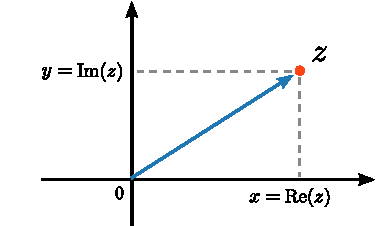
\includegraphics[width=0.45\textwidth]{complex_plane}
\end{figure}

\subsubsection{Polar representation}
\label{polar-representation}

A point in the complex plane can also be represented using polar
coordinates. Given $z = x + i y$, we can introduce polar coordinates
$r$ and $\theta$ (both real numbers):

\begin{figure}[ht]
  \centering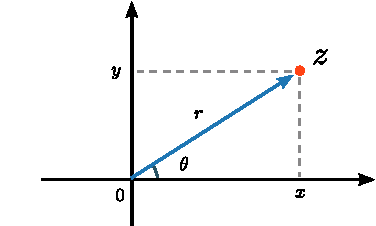
\includegraphics[width=0.45\textwidth]{complex_plane2}
\end{figure}

According to the usual formulas for converting between two-dimensional
Cartesian coordinates and polar coordinates,
\begin{align}
  r &= \sqrt{x^2 + y^2}, & x &= r\cos\theta, \\
  \theta &= \tan^{-1}(y/x), & y &= r\sin\theta.
\end{align}
The radial coordinate is equal to the magnitude of the complex number,
$|z| = r$ (see Section~\ref{conjugates-and-magnitudes}).  The
azimuthal coordinate is called the \textbf{argument} of the complex
number, and is denoted by $\mathrm{arg}(z) = \theta$.

Note that the complex zero, $z = 0$, has zero magnitude and
\textit{undefined} argument.

Using Euler's formula, Eq.~\eqref{eq:euler}, we can write
\begin{align}
  z &= x + i y \\
  &= r\cos(\theta) + i r\sin(\theta)\\
  &= r \left[\cos(\theta) + i \sin(\theta)\right] \\
  &= r \, e^{i\theta}.
\end{align}
Therefore, whenever we can manipulate a complex number into a form $A
e^{iB}$, where $A$ and $B$ are real, then $A$ is the magnitude and $B$
is the argument.  This is used in the following example:

\begin{framed}\noindent
  \textit{Example}---For $z \in \mathbb{C}$, it can be shown that
  \begin{align}
    \displaystyle \big|\exp(z)\,\big| = e^{\mathrm{Re}(z)}, \quad \mathrm{arg}\big[\exp(z)\,\big] = \mathrm{Im}(z).
  \end{align}
  Proof: Let $z = x + i y$, where $x, y \in \mathbb{R}$; then
  \begin{align}
    e^{z} = e^{x + i y} = e^x \, e^{iy}.
  \end{align}
  By inspection, the magnitude of this complex number is $e^x$, and
  its argument is $y$.
\end{framed}

\subsubsection{Geometrical interpretation of complex operations}
\label{geometrical-interpretation-of-complex-operations}

Using the complex plane, we can give geometric interpretations to the basic operations on complex numbers: 

\begin{itemize}
\item Addition of two complex numbers can be interpreted as the
  addition of two coordinate vectors. If $z_1 = x_1 + i y_1$ and $z_2
  = x_2 + i y_2$, then
  \begin{align}
    z_1 + z_2 = \left(x_1 + x_2\right) + i\left(y_1 + y_2\right).
  \end{align}
  Hence, the point corresponding to $z_1 + z_2$ is obtained by adding
  the two coordinate vectors corresponding to $z_1$ and $z_2$. From
  this, we can geometrically prove a useful inequality relation
  between complex numbers, called the ``triangle inequality'':
  \begin{align}
    |z_1 + z_2| \le |z_1| + |z_2|.
  \end{align}

\item Complex multiplication can be interpreted as a scaling together
  with a rotation.  If $z_1 = r_1e^{i\theta_1}$ and $z_2 =
  r_2e^{i\theta_2}$, then
  \begin{align}
    z_1 z_2 = \left(r_1 r_2\right) \,\exp[i(\theta_1 + \theta_2)].
  \end{align}
  Hence, the point corresponding to $z_1 \, z_2$ is obtained by
  scaling the $z_1$ coordinate vector by a factor of $|z_2|$, and
  rotating it by an angle of $\theta_2$ around the origin.  In
  particular, multiplication by $e^{i\theta}$ is equivalent to a
  rotation by angle $\theta$.

\item Complex conjugation (defined in
  Section~\ref{conjugates-and-magnitudes}) is equivalent to reflection
  about the real axis.  It moves a point from the upper half of the
  complex plane to the lower half, or vice versa.
\end{itemize}

\subsubsection{Complex numbers have no ordering}
\label{complex-numbers-have-no-ordering}

The fact that complex numbers reside in a two-dimensional plane
implies that \textit{inequality relations are undefined for complex
  numbers}. This is a critical difference between complex and real
numbers.

Real numbers can be thought of as points on a one-dimensional line
(the real line). As a consequence, they can be ordered, meaning that
for any two real numbers $a$ and $b$, one and only one of the
following is true:
\begin{align}
  a < b \;\; \mathrm{OR} \;\; a = b \;\; \mathrm{OR}\;\; a > b.
\end{align}
But since complex numbers lie in a two-dimensional plane, they cannot
be compared using ``$<$'' or ``$>$''. Given complex numbers $z_1$ and
$z_2$, it is simply nonsensical to write something like $z_1 <
z_2$. (We can, however, write $|z_1| < |z_2|$, since the magnitudes of
complex numbers are real numbers.)

\subsection{Complex functions}
\label{complex-functions}

When deriving Euler's formula in Section~\ref{eulers-formula}, we
introduced \textbf{complex functions} defined by taking real
mathematical functions, like the exponential, and making them accept
complex number inputs.  Let us take a closer look at these complex
functions.

\subsubsection{Complex trigonometric functions}
\label{complex-trigonometric-functions}

As discussed in Section~\ref{eulers-formula}, the complex sine and
cosine functions are defined by the series
\begin{align}
  \begin{aligned}
    \sin(z) &= z - \frac{z^3}{3!} + \frac{z^5}{5!} - \frac{z^7}{7!} + \cdots\\
    \cos(z) &= 1 - \frac{z^2}{2!} + \frac{z^4}{4!} - \frac{z^6}{6!} + \cdots,
  \end{aligned}
  \quad\quad z\in \mathbb{C}.
\end{align}
It is important to note that the \textit{outputs} of the complex
trigonometric functions are complex numbers too.

Some familiar properties of the real trigonometric functions do not
apply to the complex versions.  For instance, $|\sin(z)|$ and
$|\cos(z)|$ are \textit{not} bounded by 1 when $z$ is not real.

We can also write the complex cosine and sine functions in terms of
the exponential:
\begin{align}
  \cos(z) &= \;\;\frac{1}{2}\left(e^{iz} + e^{-iz}\right)
  \label{eq:cosz}\\
  \sin(z) &= -\frac{i}{2}\left(e^{iz} - e^{-iz}\right).
  \label{eq:sinz}
\end{align}
This is often a convenient step when solving integrals, as shown in
the following example.

\begin{framed}\noindent
  \textit{Example}---Consider the real integral
  \begin{align}
    I = \int_0^\infty dx \; e^{- x} \, \cos(x).
  \end{align}
  One way to solve this is to use integration by parts, but another
  way is to use the complex expansion of the cosine function:
  \begin{align}
    I &= \int_0^\infty dx \; e^{- x} \,\frac{1}{2}\, \left[e^{ix} + e^{-ix}\right] \\ &= \frac{1}{2} \int_0^\infty dx \; \left[e^{(-1+i)x} + e^{(-1-i)x}\right] \\ &= \frac{1}{2} \left[ \frac{e^{(-1+i) x}}{-1+i} + \frac{e^{(-1 - i) x}}{-1 - i}\right]_0^\infty \\ &= -\frac{1}{2} \left(\frac{1}{-1+i} + \frac{1}{-1 - i}\right) \\ &= \frac{1}{2}.
  \end{align}
\end{framed}

\subsubsection{Complex trigonometric identities}

Euler's formula provides a convenient way to deal with trigonometric
functions.  Consider the addition formulas
\begin{align}
  \sin(z_1 + z_2) &= \sin(z_1) \cos(z_2) + \cos(z_1)\sin(z_2) \\
  \cos(z_1 + z_2) &= \cos(z_1) \cos(z_2) - \sin(z_1)\sin(z_2).
\end{align}
The standard proofs for these formulas are geometric: you draw a
figure, and solve a bunch of relations between the angles and sides of
the various triangles, making use of the Pythagorean formula. But
using the Euler formula, we can prove these algebraically.  For
example,
\begin{align}
  \cos(z_1)\cos(z_2) &= \frac{1}{4}\left(e^{iz_1} + e^{-iz_1}\right) \left(e^{iz_2} + e^{-iz_1}\right)\\
  &= \frac{1}{4}\left[e^{i(z_1+z_2)} + e^{i(-z_1 + z_2)} + e^{i(z_1 -z_2)} + e^{-i(z_1+z_2)}\right] \\
  \sin(z_1)\sin(z_2) &= -\frac{1}{4}\left(e^{iz_1} - e^{-iz_1}\right) \left(e^{iz_2} - e^{-iz_1}\right) \\
  &= -\frac{1}{4}\left[e^{i(z_1+z_2)} - e^{i(-z_1 + z_2)} - e^{i(z_1 -z_2)} + e^{-i(z_1+z_2)}\right].
\end{align}
Thus,
\begin{align}
  \cos(z_1) \cos(z_2) - \sin(z_1)\sin(z_2) = \frac{1}{2}\left[e^{i(z_1+z_2)} + e^{-i(z_1+z_2)}\right] = \cos(z_1 + z_2).
\end{align}
As a bonus, these addition formulas now hold for complex inputs as
well, not just real inputs.

\subsubsection{Hyperbolic functions}
\label{hyperbolic-functions}

Euler's formula also provides us with a link between the trionometric
and hyperbolic functions.  From the definition of the hyperbolic
functions (Section 0.6):
\begin{align}
  \sinh(z) = \frac{1}{2}\left(e^{z} - e^{-z}\right), \quad\; \cosh(z) = \frac{1}{2}\left(e^{z} + e^{-z}\right).
\end{align}
Comparing this to Eqs.~\eqref{eq:cosz} and \eqref{eq:sinz}, we see
that the trigonometric and hyperbolic functions are related by
\begin{align}
  \sin(z) &= -i \sinh(iz), \quad \cos(z) = \cosh(iz) \\
  \sinh(z) &= -i \sin(iz), \quad \cosh(z) = \cos(iz).
\end{align}
Using these relations, we can relate the addition formulas for
trignometric formulas to the addition formulas for hyperbolic
functions, e.g.
\begin{align}
  \cosh(z_1+z_2) &= \cos(iz_1 + iz_2) \\
  &= \cos(iz_1)\cos(iz_2) - \sin(iz_1)\sin(iz_2) \\
  &= \cosh(z_1)\cosh(z_2) + \sinh(z_1)\sinh(z_2).
\end{align}

\subsection{Trajectories in the complex plane}
\label{trajectories-in-the-complex-plane}

Suppose we have a function that takes a real input $t$ and outputs a
complex number $z(t)$. As $t$ varies, the complex number $z(t)$ forms
a curve in the complex plane, which is called the \textbf{parametric
  trajectory} of the function $z$. Each point on the curve corresponds
to the value of $z(t)$ at some $t$.

Let us study a few examples. First, consider
\begin{align}
  z(t) = e^{i\omega t}, \quad \omega \in \mathbb{R}.
\end{align}
The trajectory is a circle in the complex plane, centered at the
origin and with radius 1. To see why, observe that the function has
the form $z(t) = r(t)\,e^{i\theta(t)}$, which has magnitude $r(t) =
1$, and argument $\theta(t) = \omega t$ varying proportionally with
$t$. If $\omega$ is positive, the argument increases with $t$, so the
trajectory is counter-clockwise. If $\omega$ is negative, the
trajectory is clockwise.

\begin{figure}[ht]
  \centering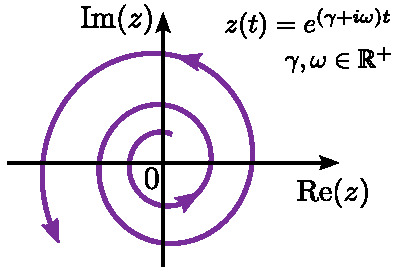
\includegraphics[width=0.37\textwidth]{complex_trajectory_2}
\end{figure}

On the other hand, consider
\begin{align}
  z(t) = e^{(\gamma + i \omega) t},
\end{align}
where $\gamma,\omega \in \mathbb{R}.$ For $\gamma = 0$, this reduces
to the previous example.  For $\gamma \ne 0$, the trajectory is a
spiral.  To see this, we again observe that this function can be
written in the form
\begin{align}
  z(t) = r(t) \;e^{i\theta(t)},
\end{align}
where $r(t) = e^{\gamma t}$ and $\theta = \omega t.$ The argument
varies proportionally with $t$, so the trajectory loops around the
origin.  The magnitude increases with $t$ if $\gamma$ is positive, and
decreases with $t$ if $\gamma$ is negative. Thus, for instance, if
$\gamma$ and $\omega$ are both positive, then the trajectory is an
anticlockwise spiral moving outwards from the origin.

Finally, consider
\begin{align}
  z(t) = \frac{1}{t + ib}, \quad b \in \mathbb{R}.
\end{align}
This trajectory is a circle which passes through the origin, as shown
below.  The center of the circle is located at $z_0 =
-i/(2b)$. Showing this requires a bit of ingenuity, and is left as an
exercise.  This is an example of something called a M\"obius
transformation.

\begin{figure}[ht]
  \centering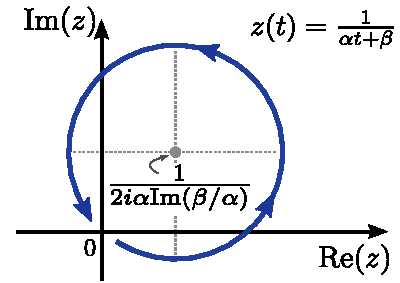
\includegraphics[width=0.37\textwidth]{complex_trajectory_3}
\end{figure}

\subsection{Why complex numbers?}\label{why-complex-numbers}

Here is a question that might have occurred to you: if we extend the
concept of numbers to complex numbers, why stop here? Why not extend
the concept further, and formulate other number systems even more
complicated than complex numbers?

As we have seen, complex numbers are appealing mathematical objects
because they can be manipulated via the same rules of algebra as real
numbers. We can add, subtract, multiply, and divide them without
running into any logical inconsistencies. One difference is that
complex numbers cannot be ordered, as discussed in
Section~\ref{complex-numbers-have-no-ordering}, but this is not a
serious limitation.

Complex numbers are, in a sense, the natural mathematical setting for
doing algebra. Arguably, they are even more advantageous than the real
numbers for doing algebra because, unlike the real numbers, they are
\textbf{algebraically closed}, meaning that all complex polynomial
equations have solutions in $\mathbb{C}$. The real numbers lack this
property: there are real algebraic equations with no solution in
$\mathbb{R}$, like $x^2 + 1 = 0$.  The algebraic closure of
$\mathbb{C}$ is called the Fundamental Theorem of Algebra, which gives
an idea of its importance (but we won't delve into the details in this
course). One consequence of this is that $\mathbb{C}$ cannot be
generalized to a more complicated number system via the same route
used to extend $\mathbb{R}$ into $\mathbb{C}$.

However, it is possible to formulate number systems more complicated
than the complex numbers, by discarding one or more of the usual rules
of algebra.  The quaternions are a system of four-component numbers
obeying an algebra that is non-commutative (i.e., $ab = ba$ is not
generally true).  The octonions are a yet more complicated system of
eight-component numbers which are not only non-commutative but also
non-associative (i.e., $(ab)c = a(bc)$ is not generally true).  These
and other number systems are occasionally useful in physics and other
fields, but overall they are vastly less important than $\mathbb{C}$.

One major reason for the usefulness of complex numbers, compared to
quaternions and octonions, is that it's relatively easy to formulate a
complex version of calculus. The concepts of derivatives and
integrals, which are defined using algebraic limit expressions, can be
more-or-less directly applied to complex functions, leading to the
subject of \textbf{complex analysis}.  We shall see later, in Chapter
7, that complex analysis has important implications for \textit{real}
calculus; for instance, many real integrals can be easily solved by
first generalizing them into complex integrals.  By contrast, since
quaternions and octonions are not commutative, the very concept of a
derivative is tricky to formulate in those number systems.

\subsection{Exercises}

\begin{enumerate}
\item
  Let $z = x + iy$, where $x, y \in \mathbb{R}$. For each of the
  following expressions, find (i) the real part, (ii) the imaginary
  part, (iii) the magnitude, and (iv) the complex argument, in terms of
  $x$ and $y$:

  \begin{enumerate}[(a)]
  \item $z^2$
  \item $1/z$
  \item $\exp(z)$
  \item $\exp(iz)$
  \item $\cos(z)$
  \end{enumerate}

\item
  Prove that $|z_1 z_2| = |z_1|\, |z_2|$, by using (i) the polar
  representation, and (ii) the Cartesian representation.
  \hfill{\scriptsize [solution~available]}

\item
  Prove that $(z_1 z_2)^* = z_1^* z_2^*$, by using (i) the polar
  representation, and (ii) the Cartesian representation.
  \hfill{\scriptsize [solution~available]}

\item
  Identify the problem with this chain of equations:
  \begin{equation*}
    -1 = i \cdot i =
    \sqrt{-1}\,\sqrt{-1} = \sqrt{-1 \cdot -1} = \sqrt{1} = 1. 
  \end{equation*}
  \vskip -0.19in
  \hfill{\scriptsize [solution~available]}

\item
  With the aid of Euler's formula, prove that
  \begin{align}
    \cos(3x) &= 4[\cos(x)]^3 -3\cos(x) \\
    \sin(3x) &= 3\sin(x)-4[\sin(x)]^3
  \end{align}

\item
  For $z_1, z_2 \in \mathbb{C}$ and $\theta \in \mathbb{R}$, show that
  $\mathrm{Re}\left[z_1 e^{i\theta} + z_2 e^{-i\theta}\right] = A
  \cos(\theta) + B \sin(\theta)$, for some $A, B \in \mathbb{R}$. Find
  explicit expressions for $A$ and $B$ in terms of $z_1$ and $z_2$.

\item
  In Section~\ref{the-complex-plane}, we saw that the conjugation
  operation corresponds to a reflection about the real axis. What
  operation corresponds to a reflection about the imaginary axis?

\item
  Consider the complex function of a real variable $z(t) = 1/(\alpha t
  + \beta)$, where $\alpha, \beta \in \mathbb{C}$ and $t \in
  \mathbb{R}$.

  \begin{enumerate}[(a)]
  \item
    For $\alpha = 1$ and $\beta = i$, show that $z(t)$ can be
    re-expressed as $z(s) = (1+e^{is})/(2i)$, where
    $s \in (-\pi,\pi)$. Hint: find a real mapping $t(s)$.

  \item
    Hence, show that the trajectory for arbitrary complex values of
    $\alpha,\, \beta$ has the form of a circle.
  \end{enumerate}

\item
  With the help of a computer plotting program, generate complex
  trajectories for the following functions (for real inputs $t
  \in\mathbb{R}$). Explain their key features, including the
  directions of the trajectories:
  \begin{enumerate}[(a)]
  \item
    $\displaystyle z(t) = \left[1+\frac{\cos(\beta t)}{2}\right] \, \exp(it)$,
    for $\beta = 10$ and for $\beta = \sqrt{5}$.
  \item
    $\displaystyle z(t) = -it \pm \sqrt{1 - t^2}$.
  \item
    $\displaystyle z(t) = ae^{it} + be^{-it}$, for $a = 1, b = -2$
    and for $a = 1, b = 2$.
  \end{enumerate}
\end{enumerate}

\end{document}
